%!TEX root = paper.tex
%
% AMRClaw
%
% Lead currently:  Marsha Berger
%

\subsection{\amrclaw} \label{sec:amrclaw}
Fortran code in the \amrclaw repository performs block-structured adaptive mesh
refinement \cite{BO,BC} for both \clawpack and \geoclaw  applications.
The algorithms implemented in \amrclaw are discussed in detail in
\cite{mjb-rjl:amrclaw,LeVequeGeorgeBerger:an11}, but a  short overview is given
here to set the stage for a description of recent changes.
\amrclaw includes the functionality for:
\begin{itemize}
\item Coordinating the flagging of points where refinement is needed,
with a variety of criteria possible for flagging cells that need refinement
from each level to the next finer level (including Richardson extrapolation,
gradient testing, or user-specified criteria)\footnote{See
\url{http://www.clawpack.org/flag.html}},
\item Organizing the flagged points into efficient grid
patches at the next finer level, using the algorithm of
\cite{mjb-rig:cluster},
\item Interpolating the solution to newly created fine grids and initializing
auxiliary data (topography, wind velocity, metric data and so on) on  these
grids,
\item Averaging fine grid solutions to coarser grids,
\item Orchestrating the adaptive time stepping (i.e. sub-cycling in time),
\item Interpolating coarse grid solution to fine grid ghost cells, and
\item Maintaining conservation at patch boundaries between resolution levels.
\end{itemize}

\amrclaw now allows users to specify ``regions'' in space-time
$[x_1,x_2] \times [y_1,y_2] \times [t_1,t_2]$ in which refinement is forced to
be at least at some level $L_1$ and is allowed to be at most $L_2$.  This can be
useful for constraining refinement, e.g. allowing or ensuring resolution of only
a small coastal region in a global tsunami simulation. Previously the user could
enforce such conditions by writing a custom flagging routine, but now this is
handled in a general manner so that the parameters above can all be specified in
the Python problem specification. Multiple regions can be specified, and a
simple rule is used to determine the constraints at a grid cell that lies in
multiple regions.

Auxiliary arrays are often used in \clawpack to store data that
describes the problem and the routine.
The routine \texttt{setaux} must then be provided by the user to set these values each time a
new grid patch is created.  For some applications computing these values can be time-consuming.  In \clawpack 5.2,
this code was improved to allow reuse of values from previous patches at
the same level where possible at each regridding time.
This is backward compatible, since no harm is done if previously
written routines are used that still compute and overwrite instead of
checking a mask.

In \clawpack 5.3 the capability to specify spatially varying boundary
conditions was added. For a single grid, it is a simple matter to
compute the location of the ghost cells that extend outside the
computational domain and set them appropriately.  With AMR however,
the boundary condition routine can be called for a grid located
anywhere in the domain, and may contain fewer or larger numbers of
ghost cells. For this reason, the boundary condition routines
 do not assume a fixed number of ghost cells.

Anisotropic refinement is allowed in both two and three dimensions.
This means that the spatial and temporal refinement ratios can be
specified independently from one another (as long as the temporal
refinement satisfies the CFL condition).  In addition, capabilities
have been added to automatically select the refinement ratio in time  on each
level based on the CFL condition.  This has only been implemented in
\geoclaw where the wave speed in the shallow water equations
depends on the local depth. The finest grids are often located only in
shallow coastal regions, so a large refinement ratio in space does not
lead to a large refinement ratio in time.

\amrclaw has been parallelized using OpenMP directives. \revised{The main
paradigm in structured AMR is an outer loop over levels of refinement, and in
inner loop overall grids at that level, where some operation is performed on
each grid (i.e. taking a time step, finding ghost cells, conservation updates,
etc.).  This inner loop is parallelized using a {\tt parallel for} loop
construct one thread is assigned to operate on one grid. Dynamic scheduling is
used with a chunk size of one.  To help with load balancing, grids at each level
are sorted from largest to smallest, using the total number of cells in the grid
as an indicator of work.} Note that this approach causes a memory bulge. Each
thread must have its own scratch arrays to save the incoming and outgoing waves
and fluxes for future conservation fix-ups. The bulge is directly proportional
to the number of threads executing. For stack-based memory allocation per
thread, the use of the environment variable {\tt OMP\_STACKSIZE} to increase the
limit may be necessary.

\cref{fig:shockbubble} shows two snapshots of the solution to a
three-dimensional shock-bubble
interaction problem found in the \clawpack \texttt{apps} repository,
illustrating localized phenomena requiring adaptive refinement.
In \cref{fig:amr_scaling} we show scalability tests and some timings for
this example, when run on a 40 core Intel Xeon Haswell machine, using
\texttt{KMP\_AFFINITY compact}.
For timing purposes, the only modifications made to the input parameters was to
turn off checkpointing and graphics output. The plot on the left shows that most
of the wall clock time is in the integration routine (\texttt{stepgrid}), which
closely
tracks the total time. The second chunk of time is in the regridding, which
contains algorithms that are not completely scalable. Very little time is in the
filling of ghost cells, mostly from other patches but also includes those at
domain boundaries. The efficiency is above 80\% until 24 cores, then drops off
dramatically. Note that there are only two level 1 grids, and an average of 22.8
level 2 grids. Most of the work is on level 3 grids, where there are an average
of 138.1 grids over all the level 3 timestep.  This is very coarse for large
numbers of cores (hence the dropoff in efficiency). At 40 cores, there are less
than 4 grids per core, and the grids are very different sizes.

\begin{figure}[t]
  \begin{center}
    \plotbox{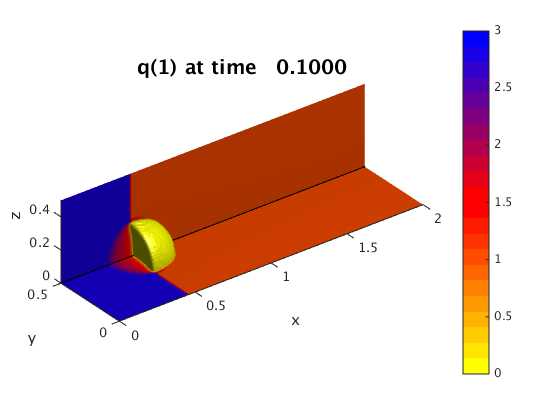
\includegraphics[width=0.45\textwidth]{f1.png}}\hfil
    \plotbox{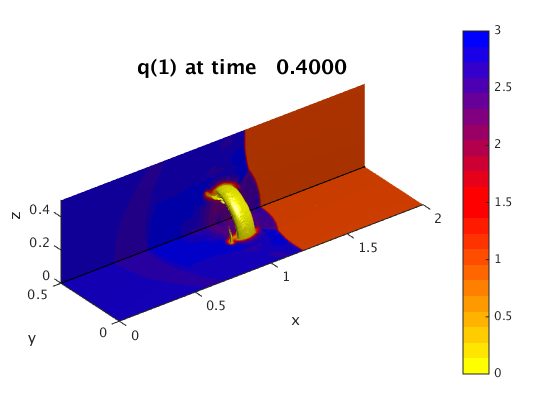
\includegraphics[width=0.45\textwidth]{f4.png}}
  \end{center}
\caption{\amrclaw example demonstrating a
  shock-bubble interaction in the Euler equations of compressible
  gas-dynamics at two times, illustrating the need for adaptive refinement
  to capture localized behavior. The
  $40\times 10\times 10$ grid at Level 1 is refined where needed
  by factors of 4 and then 2 in this 3-level run.}
\label{fig:shockbubble}
\end{figure}

\begin{figure}[h]
  \begin{center}
    % \includegraphics[width=0.45\textwidth]{amr_scaling}
    \plotbox{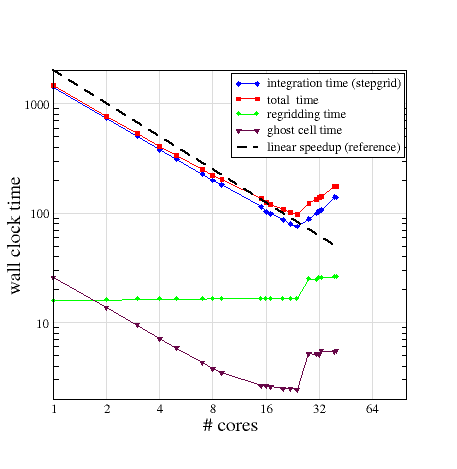
\includegraphics[width=0.4\textwidth,
      clip=true,trim=0cm 1cm 1cm 2cm]{cpuTime.png}}\hfil
    \plotbox{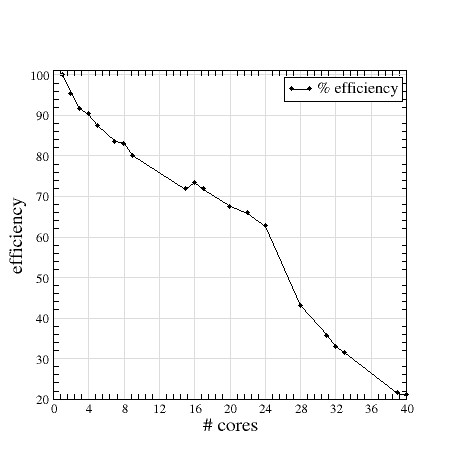
\includegraphics[width=0.4\textwidth,
      clip=true,trim=0cm 1cm 1cm 2cm]{efficiency.png}}
  \end{center}
  \caption{Left is strong scaling results for the \amrclaw example shown in
    \cref{fig:shockbubble}.
    Right is plot of efficiency based on total computational time.}
  \label{fig:amr_scaling}
\end{figure}

The parallelization of \amrclaw and \geoclaw assumes multi-core machines for the
target architecture.  \pyclaw, on the other hand, does not include AMR but uses
MPI via PETSc \revised{\cite{petsc-user-ref}} to achieve parallelism on distributed memory machines that scale
to tens of thousands of cores (see \cref{sec:pyclaw}). Other frameworks exist,
most notably \forestclaw \cite{Burstedde:we}, which are being developed in
parallel with \amrclaw, that provide scalable AMR calculations on large
distributed
memory machines.
